\documentclass[10pt]{article}
\usepackage{tmlr}
\setcitestyle{numbers}
\usepackage{amsmath,amssymb,amsthm}
\usepackage{graphicx}
\usepackage{booktabs}
\usepackage{hyperref}
\usepackage{enumitem}
\usepackage{csquotes}
\MakeOuterQuote{"}
\emergencystretch=2.5em
\sloppy

\hypersetup{colorlinks=true, linkcolor=blue, citecolor=blue, urlcolor=blue}

\title{Mean-Safe Is Not Tail-Safe: Token-Wise Latent Capacity in Multi-Head Latent Attention}
\author{\name Anonymous authors \\ \addr Paper under double-blind review}
\date{}

\begin{document}
\maketitle

\begin{abstract}
In Multi-head Latent Attention (MLA), truncating one token's cached latent changes the loss at every later position that reads it, and token-wise compression is usually judged by the mean of those changes. We measure how much of the latent a token needs for its mean loss change over the next 32 positions to stay under 0.1 nat (mean-safe), and for each of those changes to stay under 0.1 nat (worst-offset-safe). On three MLA models (30M-250M parameters) and the public DeepSeek-V2-Lite, in the latent's own coordinates, the worst-offset-safe rate is 72-79\% of the latent width. The mean criterion is nearly free: in the two of our models where we extended the rate grid to zero, about 80\% of tokens meet it with their latent content removed entirely, and the worst-offset rate is 15-20 times the mean-safe rate. On the coarser published grid the ratio is at least 6.5 at every budget from 0.05 to 0.5 nat. The gap persists under KL divergence at budgets of 0.05-0.1 nat (but falls below our criterion at 0.01), in greedy prediction flips, and in GPT-2's per-head KV cache. Its size grows with the horizon, while the worst-offset rate stays above half the latent even for the next four predictions. It does not come from a few fragile tokens: it is set by the magnitudes of the per-offset loss changes, not their signs, and these are heavy-tailed and peak just after the token. Applied jointly, mean-safe rates pass a mean-loss check while 29\% of positions exceed the budget, as many as uniform truncation at equal bytes. Rotating the latent removes about half of the worst-offset requirement in our small models but little in DeepSeek-V2-Lite. A learned router with a byte-exact packed cache ties a per-token lookup at equal bytes, and int8 quantization dominates it.
\end{abstract}

\section{Introduction}

The KV cache of autoregressive transformers [1] increasingly limits serving capacity. Multi-head Latent Attention (MLA), introduced in DeepSeek-V2 [2] and retained in DeepSeek-V3 [3], shrinks the cache by storing one low-dimensional latent per token from which per-head keys and values are reconstructed, at the same width for every token. Giving each token only the width it needs, as adaptive computation [26, 27] and per-token budget allocation in cache eviction [18, 20] do for other resources, first requires knowing what "needs" means.

A cached latent is read by every later query, so truncating it changes the loss at many future positions at once. A token can be safe in the sense that its average effect over the next $H$ positions is small, or in the stricter sense that no single future position is harmed by more than a budget $\epsilon$. We call the first mean-safe and the second worst-offset-safe (tail-safe, in the title's shorthand); a token's latent capacity requirement is the smallest latent width that keeps it safe. Compression methods are usually evaluated in the first sense, by mean loss or perplexity. Work that looks past the mean usually frames the risk as rare, extreme cases: cache entries that matter to only a few queries [38], or requests whose quality degrades materially [62]. Measured per token, the two senses are far apart for almost every token. Truncating a token's latent changes its future losses by amounts dispersed around a near-zero mean, so the mean criterion is met with almost no latent at all while safety at every offset needs most of it.

That averages can hide damage is not new: there is prior evidence from answer flips at matched accuracy [34], aggregate perplexity [35, 36], instruction following under KV-cache compression [37], per-request risk control [62], and eviction scoring and risk analysis that look past the mean [38, 39, 52]. Per-token truncation of a nested prefix is not new either: DynaKV [40] learns it outside MLA, and MatryoshkaKV [41] trains nested projections. What we add is the size of the gap inside MLA's latent, measured per cached token across future offsets; controls for what produces it; and a joint per-position test of what a mean-loss evaluation misses. Our contributions are:

\begin{itemize}

\item \textbf{The gap and its robustness} (Sections 5.1-5.2). On three MLA models spanning an 8x parameter range and on DeepSeek-V2-Lite, at $\epsilon=0.1$ nat and $H=32$, the worst-offset-safe rate is 72-79\% of the latent width in its own coordinates. The mean-safe rate is 7-9\% on our published grid, which starts at rate 16; extending the grid to zero at 30M and 250M lowers it to about 4\%, with about 80\% of tokens mean-safe at rate 0, and puts the ratio at 15-20. On the published grid the ratio is at least 6.5 at every budget from 0.05 to 0.5 nat; it is about 4.5 under KL divergence at 0.05 nat (2.4-2.6 at 0.01) and 6.2 in GPT-2's per-head KV cache. The ratio grows with the horizon $H$; the worst-offset rate barely does.

\item \textbf{What the gap does and does not reflect} (Sections 5.2-5.3). It is not a few fragile tokens: at the mean-safe rate 93-96\% of tokens exceed the budget at some offset, because gains and losses cancel in the mean. Gaussian draws matched to each probe's mean and spread account for most of the worst-offset rate (0.62-0.66 against 0.72 at 250M); keeping each probe's absolute deviations while randomizing their signs, with one draw per probe (post hoc), comes within 0.03 of it, so the magnitudes of the changes, not their signs, carry the requirement. Equal-norm noise shaped like the latent (exploratory) costs about as much as truncation on average, isotropic noise less, and neither predicts which tokens need most.

\item \textbf{The consequence} (Section 5.4). Applied jointly to 32 of the 384 positions in each 250M sequence, mean-safe rates pass a mean-loss check (+0.10 nat) while 29\% of positions exceed the budget, as many as uniform truncation at the same bytes. Worst-offset-safe rates leave 4.4\% of positions over budget, half of what uniform truncation does at their bytes.

\item \textbf{A basis caveat} (Section 5.5). The coordinate-basis rates overstate what a principal-direction truncation, the usual choice in low-rank KV compression, needs by about 50 points in our models but by 11 in DeepSeek-V2-Lite, where the requirement is mostly a property of the latent itself.

\item \textbf{A byte-exact case study} (Section 6). A pre-registered contextual router with a variable-width packed cache beats exact-byte random placement in three of four configurations but does no better than a per-token lookup table (ties in three, loses in one), and int8 quantization of the latent dominates it on bytes.

\end{itemize}

We do not claim serving gains. The packed cache stores 60-69\% of the bytes of a full MLA cache, with no peak-memory or throughput gain and a 2.4x decode-latency cost (Appendix F).

\section{Background and Related Work}

\subsection{Multi-head Latent Attention}

For hidden state $h_t$, MLA computes a compressed KV latent

\[c_t = W_{DKV}h_t \in \mathbb{R}^{d_c},\]

and reconstructs content keys and values as $W_{UK}c_t$ and $W_{UV}c_t$. A separate rotary key $k_t^R \in \mathbb{R}^{d_R}$ carries positional information. A fixed-width MLA cache stores $(c_t,k_t^R)$ instead of per-head keys and values; for sequence length $T$, $L$ layers and element size $b$ its leading storage term is $bTL(d_c+d_R)$. MLA continues work that shares or compresses key-value heads [22, 23]. Several methods convert pretrained models to MLA [4, 6, 8, 42, 43], gate latent content [7], or combine latent compression with layer sharing and quantization [5]. A mechanistic study of a small MLA model finds that the latent carries content rather than position and that, by SVD effective rank, it uses about 46\% of its width [9]. All of these keep one latent width per layer for every token.

\subsection{KV-cache compression and adaptive allocation}

KV-cache compression methods differ in which axis they compress. Eviction keeps a subset of tokens [10, 11, 12, 19], with budgets that can differ by head or layer [13, 18, 20, 44]. Quantization lowers the precision of every cached element [14, 15] or keeps important tokens at higher precision [45]. Low-rank methods project keys and values into a smaller space, uniformly or with layer-wise ranks [16, 17, 21, 46, 47], or combine decorrelation with quantization [48]; others merge states across layers [24] or learn per token whether to append or merge [25]. RateQuant [54] allocates KV-cache bit widths by rate-distortion theory, and Kim [65] bounds the per-token memory of suffix-only cache policies in a sequential source-coding frame. Adaptive computation [26, 27] likewise learns where to spend a discrete budget.

\textbf{Evaluation beyond the mean.} Dutta et al. [34] find answer flips at matched accuracy and propose KL divergence and flips as metrics; perplexity misses losses on knowledge-intensive tasks [49] and at key tokens [35], may not exercise the compressed cache at all [36], and per-sample, benchmark and long-context evaluations expose task- and instruction-dependent losses [37, 50, 51, 66]. Kang et al. [62] certify eviction policies against a per-request risk target, because a small average loss can hide requests that degrade materially. For allocation, DefensiveKV [38] aggregates each entry's importance by its maximum over observed queries instead of the mean, CriticalKV [52] scores entries by worst-case output perturbation, and Haverbeck et al. [39] analyze compression risk in minimax terms. We do not claim the observation; we measure it per cached token across future offsets.

Unlike the compression methods above, we keep every token and every head, and vary the \textit{width} of each token's latent through a nested prefix, the same nesting idea as Matryoshka representations [30] and of MatryoshkaKV [41]. The closest prior method is DynaKV [40], which learns a per-token, per-layer truncation of a PCA-initialized prefix outside MLA, continues pretraining for 128M tokens, and reports perplexity and benchmark scores, without a tail measure, above fixed-rank baselines (Palu, MatryoshkaKV). TriRoute [63] learns a per-token, per-layer KV-cache bit width jointly with attention and expert routing. Our design makes per-token rate the only thing that varies, which lets us measure how much each token needs and compare allocation policies at byte-identical budgets.

\section{Token-Wise Latent Rates}

\subsection{Nested latent prefixes}

For each layer $\ell$, calibration orders the $d_c$ latent channels by gradient-times-activation saliency, $s_{\ell,i}=\sum_t\lvert(\partial\mathcal L/\partial c_{\ell,t,i})\,c_{\ell,t,i}\rvert$ summed over calibration tokens, giving a permutation $\pi_\ell$. A token assigned rate $r_t$ keeps the nested prefix

\[\tilde c_{\ell,t}=c_{\ell,t}[\pi_\ell(1:r_t)]\]

and the remaining channels are zero. The decoupled RoPE key is never truncated. Section 6 stores such prefixes in a packed cache whose bytes depend on the rates only through their sum.

\subsection{Safe rates}

The rate $r_t$ is not an intrinsic rank: rotating the latent while compensating the up-projections ($c\mapsto Qc$, $W_U\mapsto W_UQ^{-1}$) leaves the full model unchanged but not its truncations. $r_t$ is therefore an operational rate in a chosen ordering of directions, and Section 5.5 measures how much that choice matters.

Let $\Delta_{t,j}(r)$ be the signed change in next-token cross-entropy at future offset $j\in\{0,\ldots,H-1\}$ when the latents of source token $t$, in every layer, are replaced by their rate-$r$ prefixes and every other token is kept at full width. Offset $j=0$ is the prediction made at position $t$ itself, the first one the truncated latent can affect. For a tail count $k$, let $A_{t,k}(r)$ be the mean of the $k$ largest of the $H$ values $\Delta_{t,j}(r)$. This is the empirical conditional value-at-risk [33] of the future-loss vector at level $\alpha=1-k/H$: $k=H$ gives the signed mean and $k=1$ the maximum. Tilted empirical risk [53] interpolates between the same two ends. Define the suffix-safe rate

\[r^*_{t,k}(\epsilon)=\min\{r\in\mathcal R: A_{t,k}(r')\le\epsilon\ \text{for every}\ r'\in\mathcal R,\ r'\ge r\},\]

the smallest rate from which every larger rate on the grid $\mathcal R$ is also safe (the suffix rule). With the signed mean we call $r^*$ the mean-safe rate; with the maximum, the worst-offset-safe rate.

The two criteria answer different questions. The mean criterion bounds the token's total effect over the horizon: it allows a summed loss increase of up to $H\epsilon$, spread in any way, and gains at some offsets offset harm at others. The worst-offset criterion bounds the effect on each prediction. In sequential decoding a single changed prediction can change the rest of the continuation, so the second is the one a per-position quality guarantee needs. Section 5.2 reports both criteria under KL divergence and greedy flips, which cannot offset.

\textit{Remark (ordering).} The mean of the $k$ largest elements of a fixed vector cannot decrease as $k$ shrinks, so $r^*_{t,k}(\epsilon)$ is nondecreasing as $k$ falls from $H$ to 1, for every token, budget and grid, including the nonmonotone rank-loss curves we observe (Appendix G). The spectra of Section 5 are therefore monotone by construction. The finding is their width; Section 5.2 tests how much of that width any dispersed vector would produce.

\subsection{Measuring safe rates}

For each probed source position $t$ and each rate $r$ on the grid, we zero the channels outside the layer's prefix at position $t$ in every layer simultaneously, keep every other position at full width, and record $\Delta_{t,j}(r)$ for $j=0,\ldots,H-1$. We use $H=32$ and $\epsilon=0.10$ nat unless stated otherwise. $H$ is a convention fixed before the first run, not a property of the model: the mean-safe rate falls as $H$ grows while the worst-offset rate barely moves, so we report how the ratio depends on $H$ (Section 5.2). Probe positions are drawn uniformly without replacement, 32 per sequence, from the positions whose full horizon fits in the context. Calibration data, calibration windows and evaluation windows do not overlap. The rate grid runs from 16 to $d_c$ in steps of 16 up to 64 and steps of 32 thereafter, so every requirement is resolved up to full width; Section 5.1 extends it below 16. We report, for each tail count $k\in\{32,16,8,4,2,1\}$, the mean of $r^*_{t,k}$ over probes divided by $d_c$, and the tail-capacity premium $\mathrm{TCP}=\mathbb E[r^*_{t,1}- r^*_{t,32}]/d_c$, the average extra width a token needs to be safe at its worst offset rather than on average. A positive-part criterion replaces $A_{t,H}$ by the mean of $\max(\Delta_{t,j},0)$ over the horizon, so that gains at some offsets cannot cancel harm at others.

\section{Experimental Setup}

\subsection{Models and data}

We train three decoder-only MLA language models on TinyStories [29], spanning an 8x parameter range.

\begin{table}[t]
\centering
\caption{The three MLA language models trained for this study, all on TinyStories.}
\resizebox{\textwidth}{!}{%
\small
\begin{tabular}{crrrrrrrr}
\toprule
Model & Parameters & Layers & $d_{model}$ & Heads & $d_c$ & $d_R$ & Context & Training tokens \\
\midrule
MLA-30M & 30.6M & 6 & 384 & 6 & 256 & 32 & 256 & 24.6M \\
MLA-122M & 122.14M & 12 & 768 & 12 & 384 & 32 & 384 & 147.5M \\
MLA-250M & 249.27M & 16 & 1024 & 16 & 512 & 32 & 384 & 55.3M \\
\bottomrule
\end{tabular}
}
\end{table}

Final validation losses are 1.9618 (30M), 1.5662 (122M) and 1.6588 (250M); each model is used at its final training step. The 250M model saw fewer tokens than the 122M model and has a higher loss, so every cross-scale comparison in this paper confounds size with training budget. Each scale is probed on 24 held-out sequences with 32 positions each (768 probes).

To test the findings outside our own training runs, we apply the same probe to the public DeepSeek-V2-Lite checkpoint [2]. It caches exactly the object studied here: a 512-wide latent, the same $d_c$ as our 250M model, plus a 64-wide RoPE key, in a 27-layer model with 15.7B total and 2.4B active parameters. We train nothing on it. Its text is WikiText-103 [31]: 24 test sequences of 512 tokens after a never-probed BOS token, 16 positions each (384 probes), with 32 training sequences for calibration. The latent is truncated at every layer through a forward hook on the normalization whose output the cache stores; the RoPE key is left intact. In float16 on two T4 GPUs every basis reproduces the unmodified loss (2.14 nats) exactly at full width.

\subsection{Statistical protocol}

The unit of inference is a sequence. Intervals are 95\% sequence-cluster bootstrap intervals, and comparisons between methods measured on the same probes or sequences use paired differences. The budget sweep, the equal-norm and order-statistic nulls, the KL and greedy-flip spectra, the joint-allocation test and its rate-matched references, the extended low-rank grid, and the quantization comparisons were specified with their decision rules in a committed plan before they were run (\texttt{notes/\allowbreak 2026-11-14\_tmlr\_resubmission\_plan.md}). Analyses added afterwards are labeled: a covariance-shaped null, added before any of its results were seen, is exploratory, and the horizon, offset-location and shared-draw analyses of Section 5.2 were computed from stored records in response to an internal review and are post hoc. Decision rules compare point estimates with fixed thresholds; we report intervals beside them and make no correction for multiplicity across budgets, tail levels, models and metrics, so the results are descriptive. For the router, each configuration's policy, sampling seed, 24 fresh evaluation sequences, control repeats, primary endpoint and success rule were frozen in a committed protocol before its confirmation run, and an independent audit script recomputes every router statistic from the stored per-sequence rows. Appendix B gives the protocol and its two documented departures from a clean pre-registration.

\section{Mean-Safe Is Not Tail-Safe}

\subsection{Safe rate against tail level}

\begin{table}[t]
\centering
\caption{Mean suffix-safe rate as a fraction of $d_c$ at each tail level ($\epsilon=0.10$ nat, $H=32$), in the saliency-ordered coordinate basis, on the published grid (smallest rate 16). The last rows give the share of probes whose mean criterion is met at that smallest rate, and the mean-safe rate when the grid is extended to $\{0,1,2,4,8\}$ (pre-registered; run where per-probe inputs were available). Monotonicity in $k$ holds by construction (Section 3.2). TCP is the tail-capacity premium.}
\resizebox{\textwidth}{!}{%
\small
\begin{tabular}{rrrrrr}
\toprule
$k$ (of 32) & $\alpha=1-k/H$ & 30M & 122M & 250M & DeepSeek-V2-Lite \\
\midrule
32 (mean) & 0.000 & 9.00\% & 8.22\% & 7.15\% & 8.22\% \\
16 & 0.500 & 21.47\% & 23.00\% & 22.12\% & 22.92\% \\
8 & 0.750 & 39.65\% & 39.52\% & 38.60\% & 40.14\% \\
4 & 0.875 & 55.75\% & 54.22\% & 54.16\% & 56.86\% \\
2 & 0.938 & 66.94\% & 65.56\% & 64.95\% & 70.69\% \\
1 (max) & 0.969 & 74.07\% & 72.92\% & 71.78\% & 78.65\% \\
TCP &  & 0.651 & 0.647 & 0.646 & 0.704 \\
Mean criterion met at rate 16 &  & 87\% & 83\% & 81\% & 72\% \\
32 (mean), extended grid &  & 3.77\% &  & 4.67\% &  \\
Mean criterion met at rate 0 &  & 82\% &  & 78\% &  \\
\bottomrule
\end{tabular}
}
\end{table}

To keep its average future-loss increase under 0.1 nat, a token needs on average 7-9\% of the latent on the published grid; to keep the increase under 0.1 nat at each of its next 32 positions, it needs 72-79\%. The first number is mostly the grid's smallest rate: 81-87\% of probes in our models, and 72\% on DeepSeek-V2-Lite, meet the mean criterion there. Extending the grid below 16 at 30M and 250M (pre-registered; the rate-16 losses reproduce the published ones on every probe) lowers the mean-safe rate to 3.8\% and 4.7\%. For 82\% and 78\% of probes the mean criterion is met at rate 0, with all of the token's latent content removed: the token keeps its RoPE key, so it still receives attention, but contributes no content to keys or values. The worst-offset rate does not change (71.7\% at 250M). On the extended grid the ratio is about 20 at 30M and 15 at 250M (at 30M against the published-grid worst-offset rate, which the extension could lower by at most 0.004); on the published grid it is 8.2 and 10.0, lower bounds. The premium at $\epsilon=0.10$ is 0.6507 (95\% CI [0.6326, 0.6669]) at 30M, 0.6470 ([0.6283, 0.6652]) at 122M and 0.6464 ([0.6257, 0.6665]) at 250M (Figure 1(a)). The three intervals overlap, but the agreement is a statement about the upper tail: the mean-criterion end of the premium sits at a grid floor that is a different fraction of $d_c$ in each model.

DeepSeek-V2-Lite gives a similar spectrum, somewhat heavier at the far tail. Its premium, 0.704 (95\% CI [0.676, 0.731]), is above the 0.646-0.651 of our three models and the intervals do not overlap, so we claim a similar shape and magnitude, not the same value; its mean-safe rate is an upper bound and its premium a lower bound.

The gap is not specific to MLA's latent or to our TinyStories models. In GPT-2 [32], which caches per-head keys and values, a pre-registered probe truncates the probe token's cached keys and values, in every head and layer, to a prefix of that head's principal directions, on 768 WikiText-2 [31] positions with the same $H$ and $\epsilon$. The mean-safe rate is 0.114 of the head width (95\% CI [0.105, 0.125]; 74\% of probes at the grid's smallest rate, 4 of 64) and the worst-offset rate 0.705 ([0.687, 0.723]), a ratio of at least 6.2. Because this probe truncates in principal directions, its absolute rates compare with the rotated-basis rates of Section 5.5, not with Table 2.

\begin{figure}[t]

\centering

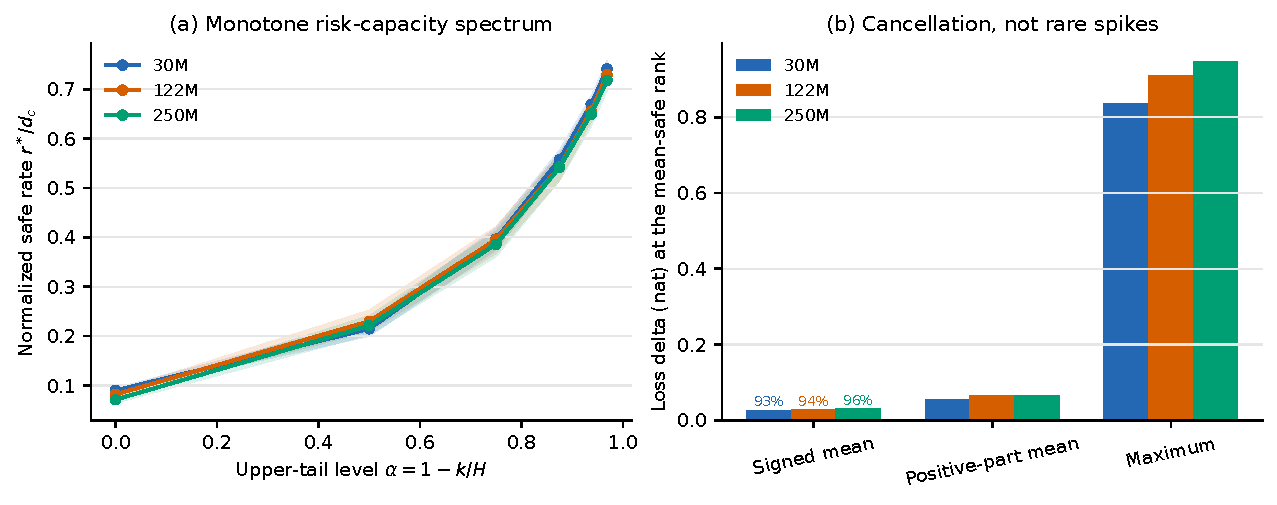
\includegraphics[width=\textwidth]{figures/elasticmla_risk_spectrum.pdf}

\caption{(a) Normalized suffix-safe rate against upper-tail level $\alpha=1-k/H$ for the three trained models on the published grid, with paired sequence-bootstrap 95\% bands; monotonicity holds by construction (Section 3.2). (b) Signed mean, positive-part mean and maximum loss change at the rate that is safe under the signed-mean criterion, annotated with the fraction of probes having at least one future offset above $\epsilon$; the gap between the signed and positive-part means is cancellation, not rare spikes.}

\label{fig:elasticmla_risk_spectrum}

\end{figure}

\subsection{What the gap does and does not reflect}

The mean of the $k$ largest of 32 signed values grows as $k$ shrinks for any vector, and per-token cross-entropy moves by more than 0.1 nat under many small perturbations. Part of the gap could therefore be produced by the budget, the horizon, the metric, the rate axis, dispersion alone, or perturbation size rather than truncation. We test each in turn.

\textbf{Budget.} Table 3 recomputes the endpoints from the stored per-offset records of the 250M model and DeepSeek-V2-Lite at four budgets; at $\epsilon=0.10$ it reproduces Table 2 exactly. The pre-registered criterion for a large gap, a worst-offset rate at least 3 times the mean-safe rate, holds at every budget on both models, with ratios of 6.5-12.8 on the published grid. These ratios are lower bounds: the share of 250M probes whose mean criterion is met at the grid's smallest rate grows from 66\% at $\epsilon=0.05$ to 81\%, 95\% and more than 99\% at 0.10, 0.20 and 0.50, which is also why the ratio stops rising at 0.50. The absolute premium is budget-specific: at 250M it falls from 0.733 at $\epsilon=0.05$ to 0.231 at $\epsilon=0.50$.

\begin{table}[t]
\centering
\caption{Mean suffix-safe rate (fraction of $d_c$) under the mean ($k=32$) and worst-offset ($k=1$) criteria at four budgets, recomputed from stored per-offset records on the published grid (smallest rate 0.031). Ratio is max over mean; because most mean-criterion rates sit at the grid floor, each ratio is a lower bound.}
\resizebox{\textwidth}{!}{%
\small
\begin{tabular}{rrrrrrrrr}
\toprule
$\epsilon$ (nat) & 250M mean & 250M max & Ratio & TCP & DSV2-Lite mean & DSV2-Lite max & Ratio & TCP \\
\midrule
0.05 & 0.133 & 0.866 & 6.5 & 0.733 & 0.139 & 0.935 & 6.8 & 0.796 \\
0.10 & 0.071 & 0.718 & 10.0 & 0.646 & 0.082 & 0.787 & 9.6 & 0.704 \\
0.20 & 0.040 & 0.514 & 12.8 & 0.474 & 0.048 & 0.549 & 11.5 & 0.501 \\
0.50 & 0.031 & 0.263 & 8.4 & 0.231 & 0.032 & 0.276 & 8.7 & 0.244 \\
\bottomrule
\end{tabular}
}
\end{table}

\textbf{Horizon.} The mean criterion averages over $H$ offsets, so it loosens as $H$ grows; the worst-offset criterion does not. Table 4 recomputes both rates at 250M with only the first $H'$ offsets of each probe, and from the separate $H=128$ run (post hoc). The worst-offset rate rises slowly, from 0.547 at $H'=4$ to 0.743 at $H'=128$, while the mean-safe rate falls from 0.238 to 0.032, so the ratio grows from 2.3 to 23. Every ratio we quote is a value at $H=32$. What is stable across horizons is the worst-offset requirement itself: on average a token must keep more than half of its latent to be safe at each of even its next four predictions. The binding offsets come early. At the grid rate just below each probe's worst-offset-safe rate, where that criterion binds, the largest loss change falls at offset $j=1$ for 20\% of probes and within the first four offsets for 49\%, against 3\% and 13\% if the worst offset were uniform; excluding $j=0$ leaves the worst-offset rate almost unchanged (0.700).

\begin{table}[t]
\centering
\caption{Effect of the horizon at 250M (post hoc): mean suffix-safe rate under the mean ($k=H'$) and worst-offset ($k=1$) criteria using the first $H'$ offsets, with the share of probes whose mean criterion is met at the grid floor. Rows marked * come from the separate $H=128$ run, whose probe positions differ.}
\resizebox{\textwidth}{!}{%
\small
\begin{tabular}{rrrrr}
\toprule
$H'$ & Mean-safe & Worst-offset-safe & Ratio & Mean criterion at floor \\
\midrule
4 & 0.238 & 0.547 & 2.3 & 51\% \\
8 & 0.181 & 0.639 & 3.5 & 59\% \\
16 & 0.122 & 0.690 & 5.6 & 68\% \\
32 & 0.071 & 0.718 & 10.0 & 81\% \\
32* & 0.065 & 0.716 & 11.0 & 84\% \\
64* & 0.040 & 0.731 & 18.2 & 94\% \\
128* & 0.032 & 0.743 & 23.2 & 99\% \\
\bottomrule
\end{tabular}
}
\end{table}

\textbf{Cancellation criterion.} If the gap came only from letting gains at some offsets cancel harm at others, a criterion that counts only harm would close it. At 250M the positive-part criterion of Section 3.3 needs 0.103 of $d_c$, against 0.071 for the signed mean and 0.718 for the worst offset.

\textbf{A metric that cannot offset.} The change in target-token cross-entropy can be negative. The KL divergence from the full model's next-token distribution to the truncated one cannot. On the same 30M and 250M probes we recomputed $r^*$ with the per-offset KL in place of the loss change, at a pre-registered primary budget $\delta=0.05$ nat (Table 5). The worst-offset rate is 4.50 times the mean-safe rate at 30M (0.490 against 0.109 of $d_c$) and 4.58 times at 250M (0.451 against 0.099), which meets the pre-registered criterion of at least 3 but is about half the ratio under the signed loss. These are lower bounds too (81\% and 70\% of probes at the floor). At $\delta=0.10$ the ratios are 4.53 and 5.84. At $\delta=0.01$, the least floored budget (35\% and 30\%), the ratios fall to 2.58 and 2.44, below the criterion. Greedy predictions, which Dutta et al. [34] propose as a metric alongside KL, show the same pattern. At the loss-based mean-safe rate, 74.6\% (30M) and 77.3\% (250M) of probes change the greedy token at least once within 32 offsets (4.4\% and 5.3\% of all offsets); at the worst-offset-safe rate, 19.1\% and 25.0\% do. Flips are sensitive to near-ties: at 250M, dropping only the last 6.25\% or 12.5\% of the channels already flips 13.4\% and 20.7\% of probes. As a rough floor, quantizing every latent at 250M to int4 changes 2.0\% of greedy predictions and to int8 0.07\% (all positions perturbed at once, so not directly comparable), against 5.3\% of offsets at the mean-safe rate and 1.0\% at the worst-offset-safe rate.

\textbf{Bit width as the rate axis.} If the gap were specific to removing channels, it would vanish on another rate axis. Quantizing only the probe token's latent (pre-registered), the smallest safe bit width rises from 1.0 bits under the mean criterion to 2.8-2.9 bits at the worst offset; the 1.8-bit gap is inconclusive by our pre-registered thresholds and a lower bound (Appendix H).

\textbf{Order statistics.} To ask how much of the worst-offset requirement dispersion alone implies, we replaced, for each 250M probe and rate, the 32 deltas by 32 independent Gaussian draws with that row's own mean and standard deviation, and recomputed $r^*$ (Table 5). At $k=1$ the Gaussian null needs 0.663 of $d_c$ against the observed 0.718, a paired difference of 0.055 [0.044, 0.065], within the pre-registered 0.10. It does not match the middle of the spectrum: at $k=16$ and $k=8$ it needs 0.131 [0.120, 0.141] and 0.104 [0.093, 0.114] \textit{more} than observed. The pre-registered null also draws fresh noise at every rate, which the suffix rule penalizes, because the highest rate that fails by chance sets $r^*$; the observed rows of adjacent rates are strongly correlated. Drawing one noise vector per probe and reusing it at every rate (post hoc) lowers the Gaussian null to 0.621 at $k=1$, 0.097 [0.086, 0.109] below observed, at the pre-registered threshold. The observed rows are heavy-tailed: averaged over all probes and rates, a row's standardized maximum is 3.3 standard deviations (2.1 for 32 Gaussian draws) and its kurtosis 11.3 (3 for a Gaussian; noisy for 32 values). A null that keeps each row's absolute deviations from its mean and randomizes only their signs, with one sign vector per probe, comes within 0.035 of the observed rate at every tail level (0.027 [0.013, 0.042] at $k=1$; the observed rate stays slightly higher at $k\le8$). The spectrum is thus nearly reproduced from the magnitudes of the per-offset deviations alone, which are larger than Gaussian at a few offsets and concentrated early in the horizon: which offsets gain and which lose hardly matters. This identifies what the requirement depends on, not where the large deviations come from.

\textbf{Equal-norm perturbations.} At 30M and 250M we replaced truncation by a perturbation of the same size, adding to the full latent, in all layers at once, a random vector with the norm of that layer's discarded channels. One direction is drawn per probe and layer and kept fixed while its norm follows the truncation schedule over the rate grid. Under the mean criterion this comparison is not informative: truncation's mean-safe rate is already within 0.04 of the grid floor, and the isotropic null sits at the floor (0.0625 at 30M, 0.031 at 250M). At $k=1$ the pre-registered isotropic null needs 0.566 and 0.434, which is 0.175 [0.148, 0.202] and 0.284 [0.264, 0.304] less than truncation: at the worst offset, truncation is harsher than isotropic noise of equal norm, so the norm of what is removed does not by itself set the requirement. Because isotropic noise may fall partly in directions the up-projections ignore, we also drew the perturbation from each layer's latent covariance (exploratory). On average this null matches truncation at every tail level: at $k=1$ it needs 0.737 and 0.703 (paired differences $-0.003$ [$-0.027$, $+0.019$] and $-0.015$ [$-0.034$, $+0.005$]). It does not match per token: the per-probe correlation of its worst-offset rate with truncation's is 0.44 and 0.48, no higher than for isotropic noise (0.41 and 0.45), with a mean absolute difference of 0.21-0.22 of $d_c$. Equal-norm noise in typical latent directions is thus about as costly on average as truncation, but which directions are perturbed matters for each token. Section 5.5 shows the other side of this: in a rotated basis the same rate discards less, and the requirement falls.

\begin{table}[t]
\centering
\caption{Controls for the spectrum endpoints at $\epsilon=0.10$ nat: mean suffix-safe rate (fraction of $d_c$) under the mean and worst-offset criteria. KL rows use budget $\delta=0.05$ nat on KL(full $\Vert$ truncated). Equal-norm nulls and KL at 30M and 250M (768 probes each); order-statistic nulls at 250M from the stored records. Mean-criterion values at or near the grid floor (0.0625 at 30M, 0.031 at 250M) are upper bounds.}
\resizebox{\textwidth}{!}{%
\small
\begin{tabular}{cccrr}
\toprule
Model & Changes from & Status & $k=32$ (mean) & $k=1$ (max) \\
\midrule
30M & truncation (observed) &  & 0.090 & 0.741 \\
30M & truncation, measured by KL & pre-registered & 0.109 & 0.490 \\
30M & isotropic equal-norm perturbation & pre-registered & 0.0625 & 0.566 \\
30M & covariance-shaped equal-norm perturbation & exploratory & 0.067 & 0.737 \\
250M & truncation (observed) &  & 0.071 & 0.718 \\
250M & truncation, measured by KL & pre-registered & 0.099 & 0.451 \\
250M & isotropic equal-norm perturbation & pre-registered & 0.031 & 0.434 \\
250M & covariance-shaped equal-norm perturbation & exploratory & 0.033 & 0.703 \\
250M & Gaussian draws, each row's mean and s.d. & pre-registered & 0.108 & 0.663 \\
250M & Gaussian, one draw shared across rates & post hoc & 0.080 & 0.621 \\
250M & sign-randomized deviations & pre-registered & 0.108 & 0.758 \\
250M & sign-randomized, one draw shared across rates & post hoc & 0.084 & 0.691 \\
\bottomrule
\end{tabular}
}
\end{table}

On DeepSeek-V2-Lite the same nulls are exploratory only, because the rerun missed our pre-registered reproduction check; within that run they point the same way (Appendix H).

\subsection{The loss changes cancel; they are not rare spikes}

If the gap were caused by a few catastrophic tokens, most tokens that are safe on average would also be safe at every offset. They are not. At the rate that is safe under the mean criterion, 93.1\% (30M), 94.1\% (122M) and 96.1\% (250M) of probes still have at least one future offset whose loss increase exceeds $\epsilon$, and the positive-part mean loss is 2.05x, 2.31x and 2.15x the signed mean (Figure 1(b)). DeepSeek-V2-Lite shows the same signature: 96.6\% of probes and 2.10x. Truncating a token's latent hurts some future predictions and helps others; the signed mean is small because the two cancel, not because the harm is small. The covariance-shaped null of Section 5.2 behaves the same way: at its own mean-safe rate, 88.5\% of 30M and 89.7\% of 250M probes have an offset above $\epsilon$ (isotropic null: 73.4\% and 65.0\%). Per probe, the ratio of the two rates at 250M has a median of 22 and a 10th percentile of 3.2 on the published grid; it is at least 10 for three quarters of probes. A mean-criterion allocation therefore under-provides for almost every token at some offset, not for a few rare ones.

\subsection{Joint application: what a mean-loss evaluation would report}

Every rate above is measured by truncating one token at a time. A pre-registered test at 250M applies them jointly. It truncates all 32 probe positions (of 384) of each of the 24 evaluation sequences in every layer, each at its own mean-safe rate and then each at its own worst-offset-safe rate, keeps the other positions at full width, and measures the loss change at every position after the first probe. As references at the same bytes, a second pre-registered run gives every probe position the sequence's mean rate, rounded (uniform; equal bytes up to rounding), or permutes the sequence's own rates across its probe positions (shuffled; exactly equal bytes). All three use the published-grid rates (Table 6).

\begin{table}[t]
\centering
\caption{Joint truncation of all 32 probe positions per sequence (250M, 24 sequences, $\epsilon=0.10$ nat). "Own" uses each position's own safe rate; "uniform" and "shuffled" spend the same rate sum. The maximum is the largest single-position loss change per sequence, averaged over sequences. Brackets: 95\% sequence-bootstrap intervals.}
\resizebox{\textwidth}{!}{%
\small
\begin{tabular}{crrrr}
\toprule
Allocation & Mean probe rate & Sequence-mean loss change & Positions above $\epsilon$ & Maximum position change \\
\midrule
Mean-safe, own & 0.071 $d_c$ & +0.102 [0.093, 0.111] & 28.6\% [27.6, 29.7] & +4.64 [3.92, 5.60] \\
Mean-safe, uniform & 0.071 $d_c$ & +0.134 [0.120, 0.148] & 29.3\% [28.0, 30.8] & +6.43 [5.65, 7.33] \\
Mean-safe, shuffled & 0.071 $d_c$ & +0.138 [0.123, 0.153] & 29.1\% [27.8, 30.7] & +6.65 [5.80, 7.60] \\
Worst-offset-safe, own & 0.718 $d_c$ & $-0.005$ [$-0.007$, $-0.004$] & 4.4\% [3.8, 5.0] & +0.41 [0.32, 0.52] \\
Worst-offset-safe, uniform & 0.718 $d_c$ & +0.008 [0.005, 0.010] & 9.7\% [9.0, 10.4] & +1.15 [0.95, 1.37] \\
Worst-offset-safe, shuffled & 0.718 $d_c$ & +0.016 [0.010, 0.022] & 11.2\% [10.2, 12.1] & +2.39 [1.61, 3.35] \\
\bottomrule
\end{tabular}
}
\end{table}

Mean safety carries over to the quantity it controls: the joint sequence-mean change, +0.102 nat, is within the pre-registered limit of $2\epsilon$, so a mean-loss evaluation would accept this allocation. Yet 28.6\% of positions exceed the budget, and the worst position in a sequence loses 4.64 nat on average. That fraction is a property of the small total rate, not of how the mean criterion places it: uniform truncation at the same bytes leaves 29.3\% of positions above $\epsilon$ (paired difference $-0.7$ points [$-1.4$, $-0.1$], within our pre-registered 5-point tolerance; the interval excludes zero, so the mean criterion is very slightly better than uniform, not worse). The mean criterion does place rate usefully for the mean and the maximum (+0.102 against +0.134 nat; 4.64 against 6.43). The worst-offset criterion places it usefully for positions: at its bytes it leaves 4.4\% of positions above $\epsilon$, against 9.7\% for uniform and 11.2\% for shuffled placement (paired difference $-5.4$ points [$-6.3$, $-4.4$], past our 5-point threshold by its point estimate but not by its whole interval), with a worst position of 0.41 nat. Worst-offset safety does not fully compose either: each probe is individually safe at every offset, but jointly 4.4\% of positions still exceed $\epsilon$. For comparison, int4 quantization of every latent at every position, at about a quarter of the bytes per compressed token, leaves 5.5\% of positions above $\epsilon$ (Section 6); the two settings compress different numbers of positions, so this is a reference, not a matched comparison.

The joint test on DeepSeek-V2-Lite, at its published per-probe rates, is exploratory for the same reason as its nulls. It shows the same pattern: the mean-safe allocation changes mean loss by 0.051 nat while 22.1\% of positions exceed $\epsilon$ and the worst position loses 4.22 nat; the worst-offset-safe allocation cuts this to 2.2\% and 0.44 nat. No rate-matched references were run on it.

\subsection{How much of the tail requirement is the basis?}

Every rate above is measured in the model's own latent coordinates, ordered by saliency: a permutation, the most restricted choice of nested directions. Truncating in a principal-direction basis is the usual choice in low-rank KV compression [16, 21, 40, 41, 48], and RoLaQ rotates the MLA latent before quantizing it [58]. We reran the identical probe in rotated orthonormal bases calibrated on the same tokens: principal directions of $\mathbb E[cc^\top]$ ("pca"), eigenvectors of the first-order loss-effect form $\mathrm{sym}(\mathbb E[gc^\top])$ ("grad"), and principal directions in the metric the up-projections apply to the latent ("model metric"). The rotation is folded into the weights, so it leaves the full-width model unchanged and makes a prefix mask a projection onto the leading directions (Appendix D).

\begin{table}[t]
\centering
\caption{Worst-offset safe rate in the coordinate basis and after rotating the latent to principal directions, with the paired per-probe fall (95\% CI shown for DeepSeek-V2-Lite).}
\small
\begin{tabular}{crrr}
\toprule
Model & Coordinate basis, max & Principal directions, max & Paired fall (points) \\
\midrule
30M & 74.07\% & 23.56\% & 50.5 \\
122M & 72.92\% & 23.25\% & 49.7 \\
250M & 71.78\% & 21.89\% & 49.9 \\
DeepSeek-V2-Lite & 78.65\% & 67.34\% & 11.3 [9.1, 13.5] \\
\bottomrule
\end{tabular}
\end{table}

In our three models (Table 7) rotation removes about 50 points of the worst-offset requirement at every scale, with paired intervals far from zero; in DeepSeek-V2-Lite it removes 11.3 points, and 59 of 384 probes still need the entire latent (106 in coordinates). Rotation helps at every tail level in every model and the bases rank the same way everywhere, but the size of the effect does not transfer; a control on an ordinary per-head KV cache agrees (Appendix D).

The simplest reading is that our small TinyStories models are unrepresentatively compressible in a rotated basis, consistent with the low effective rank reported for another small MLA model [9], and that in a production-trained MLA model the tail requirement is mostly a property of the latent code itself. In a rotated basis the gap itself remains: our GPT-2 probe (Section 5.1) truncates in principal directions and still finds a ratio of 6.2, and DeepSeek-V2-Lite's principal-direction spectrum has a ratio of 13 (Appendix D). Because the deployed packed cache and the router of Section 6 both use the coordinate basis, the coordinate-basis spectrum is the one that bounds them.

\section{Case Study: A Learned Router at Exact Bytes}

Learned per-token cache allocation exists for rank [40] and for bit width [63]. We evaluate one such allocator at exactly matched bytes, as the rate-allocation setting of Section 3 suggests.

\textbf{Storage and exact-byte controls.} The packed cache stores a flat values buffer, int32 offsets, int16 ranks, an int16 channel permutation and the uncompressed RoPE key; layer 0 is always kept at full width. For a batch-one sequence its exact tensor-payload byte count is

\[M_{\text{packed}}=
b\left[Td_c+(L-1)T\bar r+TLd_R\right]
+4L(T+1)+2LT+2Ld_c,\]

where $T$ is the sequence length, $L$ the number of layers, $b$ the element size in bytes ($b=4$ here), $\bar r=T^{-1}\sum_t r_t$, and the last three terms count offsets, ranks and permutations. The only allocation-dependent term is $b(L-1)T\bar r$, so any two allocations with the same rate sum have identical cache bytes, not approximately matched ones. This is what makes the controls below exact.

\textbf{Router.} A two-layer MLP reads the state entering layer 1, already updated by full-width layer-0 attention over the context, and picks one tier for the token, shared by all later layers. It is trained with the base model frozen, through the hard deployed tiers with a straight-through estimator [28], on language-model loss plus $\lambda$ times the expected rate (Appendix A). The 30M and 250M-coarse policies use four tiers; the 122M and 250M-fine policies use 14 and 18 tiers on the grid of Section 3.3. The primary control spends the router's exact per-sequence rate sum $R=qT+m$ by giving rate $q+1$ to $m$ random positions and $q$ to the rest, averaged over 20 draws. A configuration passes when the 95\% interval of the paired router-minus-control loss lies below zero.

\begin{table}[t]
\centering
\caption{Pre-registered fresh-window confirmations of the router against exact-byte random placement, 24 sequences per configuration. Wins count sequences on which the router has the lower loss.}
\resizebox{\textwidth}{!}{%
\small
\begin{tabular}{crrrrrrc}
\toprule
Configuration & Mean rate & Bytes vs full MLA & $\Delta$loss vs full & Router $-$ random & 95\% CI & Wins & Result \\
\midrule
30M, 4 tiers & 145.78 / 256 & 68.80\% & +0.1001 & \textbf{-0.01959} & [-0.02911, -0.00938] & 20/24 & pass \\
122M, 14 tiers & 206.93 / 384 & 61.46\% & +0.1823 & \textbf{-0.03251} & [-0.04575, -0.01958] & 21/24 & pass \\
250M, 4 tiers & 317.15 / 512 & 66.82\% & +0.1158 & +0.00190 & [-0.00222, +0.00610] & 13/24 & \textbf{fail} \\
250M, 18 tiers & 278.67 / 512 & 60.19\% & +0.1659 & \textbf{-0.01165} & [-0.01911, -0.00394] & 17/24 & pass \\
\bottomrule
\end{tabular}
}
\end{table}

\textbf{Results.} The router passes at 30M and 122M (exact one-sided sign-flip $p$ = 0.00065 and 0.000049). At 250M with four coarse tiers it fails. A second 250M protocol with 18 fine tiers, designed after the coarse result was known and run on the same 24 windows, passes ($p$ = 0.0044); it is weaker evidence than a confirmation on new windows (Appendix B), and we do not combine the four into one multi-scale claim. Permuting the router's own tiers across positions is worse in every configuration (Appendix C), so placement matters. Random placement is a weak baseline, however. Given exactly the router's per-sequence bytes, simple causal rules based on position or token type lose to the router except at 250M with four tiers, but a frequency-smoothed per-token lookup table fitted to the router's own decisions does as well: it ties the router in three configurations and beats it in the fourth (exploratory, run after the confirmations; Appendix C). We have no evidence that context beyond the current token helps. The 122M and 250M-fine policies also exceed their +0.15-nat selection budget on fresh sequences (Appendix A).

\textbf{Against quantization.} On the 24 windows of Table 2, per-token symmetric absmax quantization of the latent, without tuning (RoPE key in full precision, one fp16 scale per token and layer), costs almost nothing. int8 stores the latent in 0.504 (30M) and 0.502 (250M) of its fp16 bytes, with mean loss changes within $\pm0.0001$ nat of zero and no position above $\epsilon$; int4 uses 0.254 and 0.252, with +0.0007 nat ([$-0.0010$, $+0.0022$]) and +0.0018 nat ([0.0001, 0.0035]) and 5.6\% and 5.5\% of positions above $\epsilon$. The router's packed cache stores 60-69\% of full-MLA bytes (whole cache, including the RoPE key) at +0.10 to +0.18 nat, so int8 quantization dominates it on bytes, in line with work that stores the MLA latent in FP8 [55, 56] or fewer bits [57, 58, 59, 64]. We did not test quantizing the packed cache itself, or allocating rank and bit width jointly [60]. The packed cache also brings no peak-memory or throughput gain and decodes 2.4x slower per step (Appendix F).

\section{Limitations}

\textbf{Scale and data.} Our three models are small and trained on TinyStories, with one checkpoint, one training run and one router seed each; intervals do not include training variability, and model size is confounded with training budget. The external replication on DeepSeek-V2-Lite covers the spectrum, the budget sweep and the basis ablation on one checkpoint, one text distribution and 384 probes; the router was not run on it, and its nulls and joint test are exploratory because the rerun missed the pre-registered reproduction check (Appendix H). The GPT-2 check covers only the spectrum endpoints, in principal directions of a per-head KV cache. The extended low-rank grid was run at 30M and 250M only.

\textbf{Horizon and grid.} Every ratio is a value at $H=32$ (Table 4); the stable quantity is the worst-offset rate. Most mean-safe rates sit at the smallest rate of whichever grid is used, so they are upper bounds and the ratios lower bounds.

\textbf{Metric.} The gap is measured on next-token cross-entropy and, at 30M and 250M, on KL divergence and greedy flips. Under KL it is about half as large as under the signed loss, and at $\delta=0.01$ nat it falls below our criterion. KL is itself an imperfect proxy: it measures how far the output distribution moves, not whether it gets worse, and loses predictive power among near-baseline models [61]. Greedy flips include near-ties. None of these is a task-level or generation-level evaluation.

\textbf{What the nulls show.} The equal-norm nulls are measured at 30M and 250M, with one random direction per probe and layer; the covariance-shaped null, which matches truncation on average but not per token, is exploratory. The order-statistic nulls are measured at 250M only and use each row's own mean and spread or absolute deviations, so they show that the worst-offset rate follows from the size and shape of the per-offset deviations, not where those deviations come from. Neither shows that the dropped channels are uninformative in general.

\textbf{What $r^*$ is.} Rank-loss curves are frequently nonmonotone (Appendix G), so $r^*$ is a conservative suffix rule on a discrete grid, not a smooth or uniquely identified intrinsic rank; at 250M it raises the worst-offset rate from 0.693 under a first-crossing rule to 0.718 and barely changes the mean-safe rate (0.0715 against 0.0713). It measures isolated single-token truncation; joint truncation interacts locally (Appendix E), and the joint test of Section 5.4 covers one model and one placement of 32 probes per sequence.

\textbf{Router and auditability.} The 250M-fine confirmation reused windows whose coarse-grid outcomes had been seen, the heuristic comparisons are exploratory, and we have not compared against eviction baselines or combined the packed cache with quantization. For 30M and 122M only hash-verified aggregate summaries of the spectrum were recovered, so those spectra cannot be re-audited per probe; the 250M and DeepSeek-V2-Lite raw records are kept and authenticated by hash.

\section{Conclusion}

At $\epsilon=0.1$ nat and a 32-token horizon, keeping each of a token's next 32 losses within budget costs 72-79\% of the MLA latent in its own coordinates, while keeping their mean within budget costs almost nothing. The gap holds at every loss budget we tested, under KL divergence at 0.05-0.1 nat, with greedy flips and in GPT-2's per-head KV cache, for almost every token. Its size grows with the horizon; the worst-offset requirement does not. It is carried by the magnitudes of the per-offset loss changes, not their signs. A rotated basis removes much of it in our small models but little in DeepSeek-V2-Lite.

A mean-loss check of token-wise compression therefore says little about per-position safety: applied jointly, mean-safe rates pass it while 29\% of positions exceed the budget. In practice, our learned router does no better than a per-token lookup table at equal bytes, and int8 quantization dominates it.

\begin{thebibliography}{9}

\bibitem{ref1} A. Vaswani, N. Shazeer, N. Parmar, J. Uszkoreit, L. Jones, A. N. Gomez, Ł. Kaiser and I. Polosukhin, "Attention Is All You Need," NeurIPS, 2017.

\bibitem{ref2} DeepSeek-AI, "DeepSeek-V2: A Strong, Economical, and Efficient Mixture-of-Experts Language Model," arXiv:2405.04434, 2024.

\bibitem{ref3} DeepSeek-AI, "DeepSeek-V3 Technical Report," arXiv:2412.19437, 2024.

\bibitem{ref4} T. Ji et al., "Towards Economical Inference: Enabling DeepSeek's Multi-Head Latent Attention in Any Transformer-based LLMs," ACL, 2025.

\bibitem{ref5} Z. Yang et al., "Lossless KV Cache Compression to 2\%," arXiv:2410.15252, 2024.

\bibitem{ref6} F. Meng, P. Tang, Z. Yao, X. Sun and M. Zhang, "TransMLA: Migrating GQA Models to MLA with Full DeepSeek Compatibility and Speedup," NeurIPS, 2025.

\bibitem{ref7} Z. Cai et al., "EG-MLA: Embedding-Gated Multi-head Latent Attention for Scalable and Efficient LLMs," arXiv:2509.16686, 2025.

\bibitem{ref8} Z. Zhou et al., "CARE: Covariance-Aware and Rank-Enhanced Decomposition for Enabling Multi-Head Latent Attention," ICLR, 2026.

\bibitem{ref9} D. S et al., "Through the Bottleneck: How Multi-head Latent Attention Separates Content from Position in Language Models," arXiv:2607.23054, 2026.

\bibitem{ref10} Z. Zhang et al., "H$_2$O: Heavy-Hitter Oracle for Efficient Generative Inference of Large Language Models," NeurIPS, 2023.

\bibitem{ref11} G. Xiao, Y. Tian, B. Chen, S. Han and M. Lewis, "Efficient Streaming Language Models with Attention Sinks," ICLR, 2024.

\bibitem{ref12} Y. Li et al., "SnapKV: LLM Knows What You are Looking for Before Generation," NeurIPS, 2024.

\bibitem{ref13} Z. Cai et al., "PyramidKV: Dynamic KV Cache Compression based on Pyramidal Information Funneling," arXiv:2406.02069, 2024.

\bibitem{ref14} Z. Liu et al., "KIVI: A Tuning-Free Asymmetric 2bit Quantization for KV Cache," ICML, 2024.

\bibitem{ref15} C. Hooper et al., "KVQuant: Towards 10 Million Context Length LLM Inference with KV Cache Quantization," NeurIPS, 2024.

\bibitem{ref16} C.-C. Chang et al., "Palu: Compressing KV-Cache with Low-Rank Projection," ICLR, 2025.

\bibitem{ref17} R. Zhang et al., "LoRC: Low-Rank Compression for LLMs KV Cache with a Progressive Compression Strategy," arXiv:2410.03111, 2024.

\bibitem{ref18} Y. Feng et al., "Ada-KV: Optimizing KV Cache Eviction by Adaptive Budget Allocation for Efficient LLM Inference," NeurIPS, 2025.

\bibitem{ref19} Z. Liu et al., "Scissorhands: Exploiting the Persistence of Importance Hypothesis for LLM KV Cache Compression at Test Time," NeurIPS, 2023.

\bibitem{ref20} S. Ge et al., "Model Tells You What to Discard: Adaptive KV Cache Compression for LLMs," ICLR, 2024.

\bibitem{ref21} U. Saxena et al., "Eigen Attention: Attention in Low-Rank Space for KV Cache Compression," Findings of EMNLP, 2024.

\bibitem{ref22} N. Shazeer, "Fast Transformer Decoding: One Write-Head is All You Need," arXiv:1911.02150, 2019.

\bibitem{ref23} J. Ainslie et al., "GQA: Training Generalized Multi-Query Transformer Models from Multi-Head Checkpoints," EMNLP, 2023.

\bibitem{ref24} A. Liu et al., "MiniCache: KV Cache Compression in Depth Dimension for Large Language Models," NeurIPS, 2024.

\bibitem{ref25} P. Nawrot et al., "Dynamic Memory Compression: Retrofitting LLMs for Accelerated Inference," ICML, 2024.

\bibitem{ref26} A. Graves, "Adaptive Computation Time for Recurrent Neural Networks," arXiv:1603.08983, 2016.

\bibitem{ref27} D. Raposo et al., "Mixture-of-Depths: Dynamically Allocating Compute in Transformer-Based Language Models," arXiv:2404.02258, 2024.

\bibitem{ref28} Y. Bengio, N. Léonard and A. Courville, "Estimating or Propagating Gradients Through Stochastic Neurons for Conditional Computation," arXiv:1308.3432, 2013.

\bibitem{ref29} R. Eldan and Y. Li, "TinyStories: How Small Can Language Models Be and Still Speak Coherent English?," arXiv:2305.07759, 2023.

\bibitem{ref30} A. Kusupati et al., "Matryoshka Representation Learning," NeurIPS, 2022.

\bibitem{ref31} S. Merity, C. Xiong, J. Bradbury and R. Socher, "Pointer Sentinel Mixture Models," ICLR, 2017.

\bibitem{ref32} A. Radford, J. Wu, R. Child, D. Luan, D. Amodei and I. Sutskever, "Language Models are Unsupervised Multitask Learners," OpenAI technical report, 2019.

\bibitem{ref33} R. T. Rockafellar and S. Uryasev, "Optimization of Conditional Value-at-Risk," Journal of Risk, 2(3):21-42, 2000.

\bibitem{ref34} A. Dutta, S. Krishnan, N. Kwatra and R. Ramjee, "Accuracy is Not All You Need," NeurIPS, 2024.

\bibitem{ref35} L. Fang et al., "What is Wrong with Perplexity for Long-context Language Modeling?," arXiv:2410.23771, 2024.

\bibitem{ref36} S. M. M. Murshed, H. Bright, R. Karim and A. S. Sichani, "EdgeLLM-Nano: Auditing Polar-Guided Key-Cache Compression and Consistency-Anchored Pruning on a 33.6 MB On-Device Language Model," arXiv:2610.14475, 2026.

\bibitem{ref37} A. Chen, R. Geh, A. Grover, G. Van den Broeck and D. Israel, "The Pitfalls of KV Cache Compression," ACL, 2026.

\bibitem{ref38} Y. Feng, H. Guo, J. Lv, S. K. Zhou and X. Xie, "Taming the Fragility of KV Cache Eviction in LLM Inference," arXiv:2510.13334, 2025.

\bibitem{ref39} L. Haverbeck, C. Amo Alonso, A. F. Posada-Moreno, S. Trimpe and M. Pavone, "The risk of KV cache compression," NeurIPS, 2026.

\bibitem{ref40} L. Lu et al., "One Size Does Not Fit All: Token-Wise Adaptive Compression for KV Cache," arXiv:2603.04411, 2026.

\bibitem{ref41} B. Lin et al., "MatryoshkaKV: Adaptive KV Compression via Trainable Orthogonal Projection," ICLR, 2025.

\bibitem{ref42} G. Li, M. Rezagholizadeh, M. Yang, V. Appia and E. Barsoum, "X-EcoMLA: Upcycling Pre-Trained Attention into MLA for Efficient and Extreme KV Compression," arXiv:2503.11132, 2025.

\bibitem{ref43} Z. Wang, Z. Xie and T. Ji, "MLAfication: Efficiently Enabling High-Fidelity MLA for Modern LLMs," arXiv:2610.17202, 2026.

\bibitem{ref44} Y. Fu et al., "Not All Heads Matter: A Head-Level KV Cache Compression Method with Integrated Retrieval and Reasoning," ICLR, 2025.

\bibitem{ref45} J. Y. Yang et al., "No Token Left Behind: Reliable KV Cache Compression via Importance-Aware Mixed Precision Quantization," arXiv:2402.18096, 2024.

\bibitem{ref46} Y. Xu et al., "ThinK: Thinner Key Cache by Query-Driven Pruning," ICLR, 2025.

\bibitem{ref47} C.-C. Chang et al., "xKV: Cross-Layer KV-Cache Compression via Aligned Singular Vector Extraction," ICML, 2026.

\bibitem{ref48} K. Staniszewski and A. Łańcucki, "KV Cache Transform Coding for Compact Storage in LLM Inference," ICLR, 2026.

\bibitem{ref49} A. Jaiswal et al., "Compressing LLMs: The Truth is Rarely Pure and Never Simple," ICLR, 2024.

\bibitem{ref50} J. Yuan et al., "KV Cache Compression, But What Must We Give in Return? A Comprehensive Benchmark of Long Context Capable Approaches," arXiv:2407.01527, 2024.

\bibitem{ref51} C.-P. Hsieh et al., "RULER: What's the Real Context Size of Your Long-Context Language Models?," COLM, 2024.

\bibitem{ref52} Y. Feng et al., "CriticalKV: Optimizing KV Cache Eviction from an Output Perturbation Perspective," ICML, 2026.

\bibitem{ref53} T. Li, A. Beirami, M. Sanjabi and V. Smith, "Tilted Empirical Risk Minimization," ICLR, 2021.

\bibitem{ref54} F. Zuo, Z. Zhou, H. Cong, X. Xi and H. F. Leung, "RateQuant: Optimal Mixed-Precision KV Cache Quantization via Rate-Distortion Theory," arXiv:2605.06675, 2026.

\bibitem{ref55} Y. Zhang et al., "SnapMLA: Efficient Long-Context MLA Decoding via Hardware-Aware FP8 Quantized Pipelining," arXiv:2602.10718, 2026.

\bibitem{ref56} DeepSeek-AI, "DeepSeek-V3.2: Pushing the Frontier of Open Large Language Models," arXiv:2512.02556, 2025. FP8 latent-cache layout documented in \texttt{github.com/\allowbreak deepseek-ai/\allowbreak FlashMLA}.

\bibitem{ref57} Z. Su et al., "QuantMLA: Function-Aligned Dual-Path Quantization for Low-Bit MLA KV Caching," arXiv:2609.36760, 2026.

\bibitem{ref58} S. Ji et al., "RoLaQ: Joint Rotation and Range Calibration for 2-Bit KV Caches in Multi-Head Latent Attention," arXiv:2610.20686, 2026.

\bibitem{ref59} T. Chen et al., "RAQ-MLA: Role-Aware Quantization for Multi-Head Latent Attention Caches," arXiv:2610.33625, 2026.

\bibitem{ref60} R. Krishnan and V. Schulz, "A JoLT for the KV cache: Near-Lossless KV Cache Compression via Joint Rank-bit Allocation," arXiv:2607.12550, 2026.

\bibitem{ref61} M. Nikolić, A. H. Zadeh, E. Torres Sanchez and A. Moshovos, "Displacement Is Not Direction: Evaluating Fidelity Metrics for Quantized LLM Deployment," arXiv:2606.19558, 2026.

\bibitem{ref62} B. Kang, S. Yun, H. Kim and H. Seo, "Risk-Controlled KV-Cache Eviction: From Memory Budgets to Risk Targets," arXiv:2609.27981, 2026.

\bibitem{ref63} A. Balashov and O. Ponomarova, "TriRoute: Unified Learned Routing for Joint Adaptive Attention, Experts, and KV-Cache Allocation," arXiv:2607.06601, 2026.

\bibitem{ref64} C. Ni et al., "NVFP4-MLA: Unified FP4 KV-Cache Storage and Attention Computation for Multi-Head Latent Attention," arXiv:2611.18972, 2026.

\bibitem{ref65} M. Kim, "Polynomial Context-Truncation Sensitivity in Autoregressive Language Models: Sequential Wyner-Ziv Bounds for KV Cache Compression," arXiv:2605.25085, 2026.

\bibitem{ref66} W. Gao, X. Zhou, P. Sun, T. Zhang and Y. Wen, "Rethinking Key-Value Cache Compression Techniques for Large Language Model Serving," MLSys, 2025.

\end{thebibliography}

\appendix

\section{Router training and selection details}

Layer 0 is kept at full width to avoid the circularity of compressing the state that decides the compression. Deployment uses the hard choice $y_t=\text{onehot}(\arg\max a_t)$. Training passes gradients through it with a straight-through estimator [28], $\hat y_t = y_t + p_t-\operatorname{stopgrad}(p_t)$ with $p_t=\operatorname{softmax}(a_t/\tau)$, so that the forward pass is exactly the deployed hard rollout, and minimizes

\[\mathcal J(\theta)=\mathcal L_{LM}(\hat y)+\lambda\frac{1}{Td_c}\sum_t\sum_{m}p_{t,m}\mathcal T_m\]

with the base model frozen. Isolated-token capacity labels, the obvious supervised target, are not joint-rollout labels: an early router trained on them collapsed toward the smallest tier when every token was compressed at once, and second-order interaction measurements confirm that isolated labels are misaligned with joint truncation, although only locally (Appendix E).

The 4-tier grid is $\{16,64,160,256\}$ at 30M and $\{32,128,320,512\}$ at 250M (6.25\%, 25\%, 62.5\% and 100\% of $d_c$). The fine grid runs from 16 in steps of 16 up to 64 and in steps of 32 thereafter, giving 14 tiers at 122M ($d_c=384$) and 18 at 250M ($d_c=512$). Candidate $\lambda$ values were trained on 16 sequences, and $\lambda$ was chosen on four validation sequences as the cheapest candidate within +0.15 nat of full MLA that also beat an exact-byte static control. The selected values are $\lambda=0.4$ (30M), $0.8$ (122M), $0.4$ (250M, 4 tiers) and $0.8$ (250M, 18 tiers); the two 250M policies were trained and frozen independently. The 122M and 250M-fine routers start from a random initialization; the other two start from the isolated-position supervised router. At 122M the 4-tier grid produced no candidate that beat the exact-byte static control within the validation budget, and the 14-tier grid was adopted before any fresh-window run; this is consistent with the tier-resolution explanation of Section 6, but means the 30M-coarse / 122M-fine contrast was not designed in advance. Four older development sequences were observed repeatedly during method development; they are exploratory and enter no confirmatory claim.

On fresh sequences the 30M and 250M-coarse policies stay within the +0.15-nat selection budget (+0.1001 and +0.1158 nat); the 122M and 250M-fine policies do not (+0.1823 and +0.1659, against +0.1408 and +0.1483 on validation). Budget calibration and allocation quality are separate axes: 122M misses its budget but keeps its advantage over random placement, while 250M-coarse meets its budget and loses that advantage. A deployed system would need a larger calibration set, a risk margin, or fallback to a higher tier.

\begin{figure}[t]

\centering

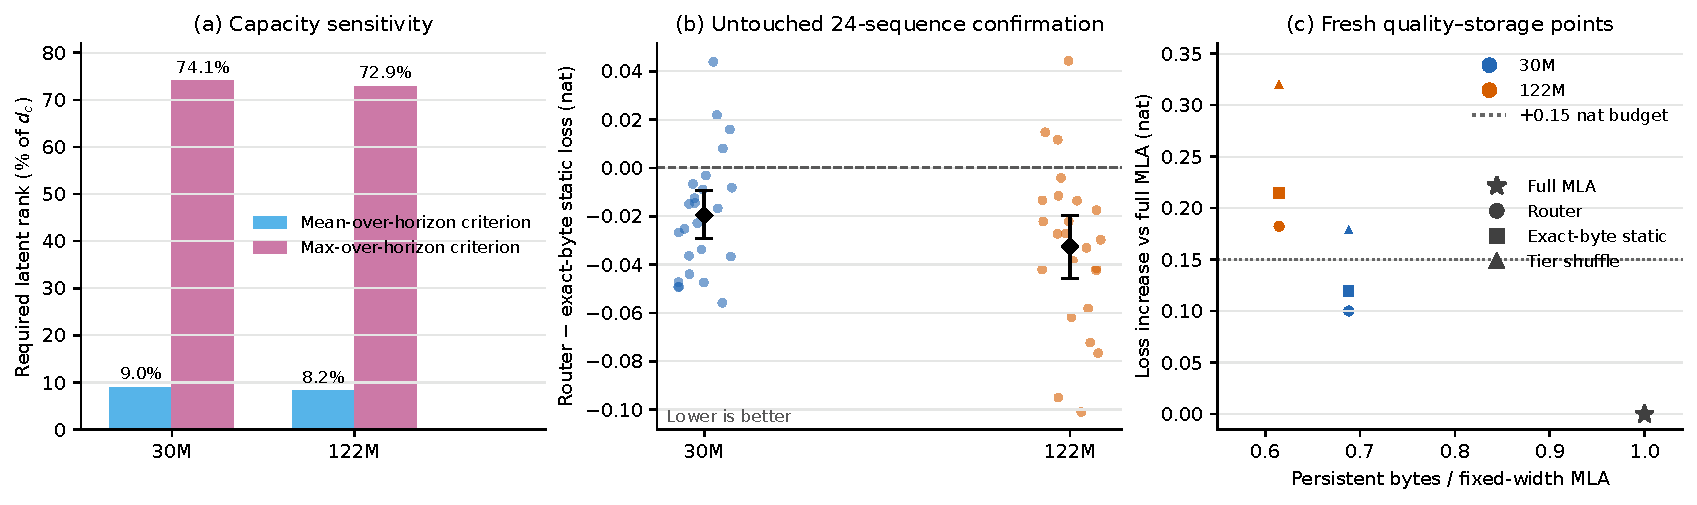
\includegraphics[width=\textwidth]{figures/elasticmla_main_results.pdf}

\caption{(a) Mean required rate under the mean and maximum criteria, averaged over 768 probes per scale. (b) Per-sequence router-minus-control loss differences at 30M and 122M; dots are sequences, diamonds means, error bars paired sequence-bootstrap 95\% intervals. (c) Mean fresh-sequence loss increase over full MLA against cache bytes; both controls have exactly the router's per-sequence bytes. Points are evaluated configurations, not an interpolated curve.}

\label{fig:elasticmla_main_results}

\end{figure}

\section{Confirmation protocol and provenance}

For 30M and 122M, commit \texttt{a4bcc7f} froze each policy file and its SHA-256 hash, the sampling seed (91,827), 24 fresh sequences, 20 control permutations, the primary endpoint and the success rule, before any fresh-window result existed (\texttt{notes/\allowbreak fresh\_confirmation\_protocol.md}). The machine-readable manifest that later scripts authenticate against (\texttt{experiments/\allowbreak fresh\_confirmation\_manifest.json}) was written afterwards, in the commit of the 30M/122M results (\texttt{080af82}); it restates the frozen values, but the oracle and summary hashes it adds were not part of the 30M/122M freeze. The 250M-coarse and 250M-fine entries were each committed to the manifest before their runs (\texttt{1ee1528}, \texttt{010e670}).

The two departures from a clean pre-registration are these. First, the 250M-fine entry was added after the 250M-coarse result was known, to test the tier-resolution explanation, and reused the same 24 windows (same seed and exclusion set). Its policy was trained and selected on the original training and validation sequences only, so the reuse cannot have tuned it, but it is a second look at windows whose coarse outcomes had been seen. Second, the original cloud commands preceded the later manifest-enforcement arguments; the frozen protocol commit, complete logs and audits bind those results, and future runs fail unless their manifest inputs match.

Fresh windows come from the held-out region and are separated from all 24 earlier oracle and development windows, and from each other, by at least \texttt{block\_size + 1} tokens. \texttt{experiments/\allowbreak audit\_fresh\_confirmation.py} reconstructs the seeded sampler and recomputes every statistic from the stored per-sequence rows; it checks sampling, byte equality and arithmetic, but does not rerun the model. \texttt{experiments/\allowbreak audit\_joint\_training\_replay.py} compared a separately retrained policy with the frozen one and found a bit-for-bit match; the retrained files were not committed, so repeating that check requires retraining. Exact one-sided sign-flip tests enumerate all sign assignments, which assumes exchangeable signs under the null.

\section{Heuristic comparison details}

The four rules are absolute position, token identity (a frequency-smoothed per-token lookup table), inverse token frequency, and coarse token type, each fitted as a predictor of the router's own tier on the 16 training sequences. Each rule scores tokens; in the main comparison (Section 6) a token gets $r_t=\lfloor s_t+\beta\rfloor$ clipped to $[1,d_c]$, with $\beta$ solved per sequence and the integer remainder given to the largest fractional parts, so that the rule spends exactly the router's rate sum without being restricted to the router's tiers. In the second variant the rule receives the router's realized tier multiset and only decides which positions get which tier (highest score, highest tier; ties broken at random and averaged over five draws), the frame of the shuffle control. Every evaluation asserts byte equality with the router.

\begin{table}[t]
\centering
\caption{Router minus rule loss (nat) for every configuration and rule, with the rule choosing its own histogram (with 95\% CI) or restricted to the router's tier multiset.}
\resizebox{\textwidth}{!}{%
\small
\begin{tabular}{ccrcr}
\toprule
Configuration & Rule & Router $-$ rule, own histogram & 95\% CI & Router $-$ rule, router's histogram \\
\midrule
30M, 4 tiers & position & -0.0225 & [-0.0326, -0.0117] & -0.0804 \\
30M, 4 tiers & token identity & +0.0024 & [-0.0079, +0.0130] & -0.0049 \\
30M, 4 tiers & token frequency & -0.0084 & [-0.0162, +0.0002] & -0.0437 \\
30M, 4 tiers & token type & -0.0146 & [-0.0241, -0.0050] & -0.0689 \\
122M, 14 tiers & position & -0.0359 & [-0.0497, -0.0227] & -0.1309 \\
122M, 14 tiers & token identity & -0.0033 & [-0.0133, +0.0065] & -0.0160 \\
122M, 14 tiers & token frequency & -0.0045 & [-0.0175, +0.0091] & -0.0418 \\
122M, 14 tiers & token type & -0.0284 & [-0.0421, -0.0151] & -0.1139 \\
250M, 4 tiers & position & +0.0012 & [-0.0031, +0.0054] & -0.0210 \\
250M, 4 tiers & token identity & +0.0045 & [+0.0012, +0.0080] & -0.0019 \\
250M, 4 tiers & token frequency & +0.0071 & [+0.0028, +0.0114] & -0.0142 \\
250M, 4 tiers & token type & +0.0009 & [-0.0035, +0.0053] & -0.0217 \\
250M, 18 tiers & position & -0.0133 & [-0.0208, -0.0050] & -0.0397 \\
250M, 18 tiers & token identity & +0.0022 & [-0.0053, +0.0100] & -0.0103 \\
250M, 18 tiers & token frequency & -0.0001 & [-0.0084, +0.0090] & -0.0164 \\
250M, 18 tiers & token type & -0.0114 & [-0.0189, -0.0039] & -0.0430 \\
\bottomrule
\end{tabular}
}
\end{table}

With its own histogram the router wins 6 of 16, ties 8 and loses 2. Restricted to the router's tier multiset the rules lose 14 and tie 2 (30M token identity and 250M-coarse token identity), but that variant handicaps them: the router chose its histogram together with its placement, and a near-uniform histogram is itself better than a shuffled router histogram (Section 6). We therefore treat the own-histogram comparison as the operative one. An earlier version of this comparison let each rule run at its own validation-selected bytes, which differed from the router's by -6.5\% to +12.9\% and decided almost every outcome by budget rather than placement; it is superseded by the byte-matched results here (\texttt{notes/\allowbreak code\_review\_2026-10\_corrections.md}).

The shuffle control of Section 6, which permutes the router's own tier multiset across positions, loses to the router by 0.07989 nat (30M), 0.13907 (122M), 0.01765 (250M, 4 tiers) and 0.03551 (250M, 18 tiers), all with intervals excluding zero.

\section{Basis ablation details}

With $W_{DKV}$, $W_{UK}$ and $W_{UV}$ bias-free, substituting $U^\top W_{DKV}$, $W_{UK}U$ and $W_{UV}U$ for an orthonormal $U$ leaves the full-width function unchanged while making a prefix mask a projection onto $\mathrm{span}(U_{:,:k})$; this is verified at full width to at most $3.1\times10^{-5}$ logit deviation. The "grad" basis uses eigenvectors of $\mathrm{sym}(\mathbb E[gc^\top])$, whose quadratic form is the mean first-order loss effect of dropping a direction; its diagonal in the coordinate basis is the signed version of the saliency used by the packed cache, so the deployed ordering is the axis-aligned special case of the same criterion. The "model metric" basis uses principal directions of $A^{1/2}\mathbb E[cc^\top]A^{1/2}$ with $A=W_{UK}^\top W_{UK}+W_{UV}^\top W_{UV}$, the frame that minimizes reconstruction error in the metric the model applies to the latent.

In our three models the worst-offset requirement under principal directions is 23.56\%, 23.25\% and 21.89\% (paired falls 50.5, 49.7 and 49.9 points). Under the coordinate basis at 30M, 410 of 768 probes need at least 224 of 256 channels, against 3 under rotation; at 250M, 77 of 768 need the full latent under coordinates and none under rotation. Ordering by first-order loss effect is worse than ordering by reconstruction at every scale (10.7, 12.5 and 10.3 points): the worst-offset criterion binds near a quarter of the width, far from where a linearization taken at full width applies. The model-metric frame wins by under a point at 30M and 250M and ties principal directions at 122M, with about half of all probes tied. Under rotated bases more probes have a nonmonotone rank curve (59\% to 82\% at 30M, 78\% to 98\% at 250M), and rotated-basis mean-criterion values sit on the grid's smallest entry and are upper bounds. The coordinate arm reproduces the main-text endpoints and histograms exactly. Table 10 gives all four bases for DeepSeek-V2-Lite.

\begin{table}[t]
\centering
\caption{DeepSeek-V2-Lite: mean suffix-safe rate as a fraction of $d_c$ in the four bases.}
\resizebox{\textwidth}{!}{%
\small
\begin{tabular}{rrrrr}
\toprule
$k$ (of 32) & coord & pca & grad & model metric \\
\midrule
32 (mean) & 8.22\% & 5.06\% & 5.94\% & 5.19\% \\
16 & 22.92\% & 12.72\% & 16.58\% & 13.79\% \\
8 & 40.14\% & 25.68\% & 31.18\% & 26.68\% \\
4 & 56.86\% & 42.36\% & 49.51\% & 43.47\% \\
2 & 70.69\% & 56.90\% & 64.97\% & 57.44\% \\
1 (max) & 78.65\% & 67.34\% & 73.47\% & 67.58\% \\
TCP & 0.704 & 0.623 & 0.675 & 0.624 \\
\bottomrule
\end{tabular}
}
\end{table}

These four bases were measured in two runs that share bit-identical evaluation tokens, probe positions and baseline losses, checked before pairing; each run computed its own calibration statistics, whose float16 GPU backward pass is not bit-deterministic.

The per-head KV control truncates the key and value of each head of an ordinary multi-head cache in coordinate and rotated bases at loss budgets of 0.05-0.5 nat. The coordinate basis overstates the required width by 1.65-3.22x on our three models but by 1.06-1.30x on GPT-2 and GPT-2-medium [32] (\texttt{notes/\allowbreak kv\_cache\_basis\_generalization.md}, \texttt{notes/\allowbreak low\_rank\_does\_not\_mean\_compressible.md}).

\section{Pairwise interaction of truncations}

Isolated-token labels would be joint-rollout labels if truncation effects were additive. We measured the second-order mixed difference $L_{\{t_1,t_2\}}-L_{\{t_1\}}-L_{\{t_2\}}+L_{\emptyset}$, which vanishes for any additive distortion, over 1008 position pairs per scale. It is nonzero, so isolated labels are structurally misaligned with joint routing, but the misalignment is local. As a fraction of the individual effects it is 9.09\%, 12.17\% and 13.17\% at 30M, 122M and 250M for adjacent positions averaged over three tested rates (16.79\%, 23.28\% and 22.78\% at rate 16 alone), decays monotonically with separation, and falls below 1.3\% beyond 32 tokens. It grows with truncation severity (5.69\% at rate 16 to 1.07\% at rate 224 at 30M, averaged over separations). We draw no scale trend: the tested rates are fixed absolute values and so different fractions of $d_c$ at each scale, and with 144 pairs per cell from eight sequences and no interval, the data neither establish nor exclude growth with scale (\texttt{notes/\allowbreak pair\_interaction\_prediction5.md}).

\section{Packed-cache memory and latency}

We benchmarked prefill followed by 128 incremental decode steps on a Tesla T4, comparing full-width dense MLA, a uniform packed cache at the router's realized mean rate, and the router's packed cache.

\begin{table}[t]
\centering
\caption{Prefill followed by 128 decode steps on a Tesla T4, router packed cache against full-width MLA. Cache bytes and decode times come from the paired append benchmark; peak memory from the later rerun with the harness fix described below.}
\small
\begin{tabular}{crrr}
\toprule
Model & Cache bytes, router / full & Peak allocated, router / full & Decode step, router (vs full) \\
\midrule
30M & 67.4\% & 99.7\% & 18.83 ms (2.42x) \\
122M & 59.6\% & 99.3\% & 42.11 ms (2.37x) \\
\bottomrule
\end{tabular}
\end{table}

Measured cache bytes track the byte formula of Section 6. Peak allocated memory is essentially unchanged, because at these model sizes and context lengths it is dominated by weights and the prefill's vocabulary-sized logits, not by the cache. Decode is 2.4x slower per step. Most of the remaining cost is the dense reconstruction of the latent before each attention call, which is inherent to a persistent representation that is packed: removing it requires computing the per-head projections directly on the ragged buffer, a kernel we have not written. We therefore claim byte-exact persistent-cache savings, not peak-memory or throughput gains.

As first written, the packed decode step was 167.9x (30M) and 201.1x (122M) slower than full MLA. Three unvectorized Python loops were responsible: \texttt{pack\_latents}, \texttt{unpack\_latents} and \texttt{append\_packed\_latents} rebuilt the whole cached history token by token on every decode step, and \texttt{forward\_cached\_packed} built its rank mask with a nested Python loop. Rewriting all three as vectorized operations cut the regression to 3.00x and 2.96x, verified by 500 random-trial cross-checks against the original implementations with zero mismatches. Reordering the flat buffer (sequence, batch) made appending a concatenation, and moving per-step defensive validation to where its guarantee is established removed the dominant remaining cost. This gives the 2.42x and 2.37x of Table 11, measured as a paired benchmark against the previous version inside one T4 job (dense control moved by 1.1\% at 30M and 0.4\% at 122M), and verified by bit-identical end-to-end decode logits, ranks and cache bytes. An earlier version of the benchmark reported a 3.5-4.2\% peak-memory reduction; it was a harness artifact (only the router path released its prefill logits before decoding) and disappears when every path does (\texttt{notes/\allowbreak measured\_cache\_memory\_latency.md}). The 30M decode runs to position 320, past its 256-token training context.

\section{Nonmonotone rank-loss curves and reproducibility}

Raw rank-loss curves are frequently nonmonotone: 83.6\%, 89.3\% and 92.1\% of mean-over-horizon curves and 59.4\%, 69.7\% and 78.0\% of max-over-horizon curves at 30M, 122M and 250M have at least one rise (the grids have 10, 14 and 18 points, so these frequencies are not comparable across scales). This is why $r^*$ uses the suffix rule. An earlier run at 250M stopped the rate grid at 384 and jumped to 512, which rounded every requirement in (384, 512] up to full width and overstated the 250M tail rates by up to 4.3 points; all 250M numbers here come from the corrected rerun with the same seeds, checkpoint, windows and channel orders. The 122M-minus-30M differences in the mean and max endpoints are -0.781 points (95\% CI [-1.617, +0.076]) and -1.156 points ([-3.849, +1.611]).

\section{Additional controls}

\textbf{Bit width as the rate axis.} In a pre-registered probe on the same 768 probes per model, we quantized only the probe token's latent, in every layer, at 1-6 and 8 bits (1 bit is the sign times the row's mean magnitude) and took the smallest safe bit width $w^*$ under the suffix rule at $\epsilon=0.10$ nat. The mean $w^*$ rises from 1.01 bits under the mean criterion to 2.85 (30M) and 2.78 (250M) at the worst offset. These gaps, 1.84 and 1.77 bits, fall between our pre-registered thresholds for absent (at most 1 bit) and present (at least 2 bits), so the reading is inconclusive; the mean criterion sits at the 1-bit floor of the axis, so both gaps are lower bounds. Per-token quantization is far cheaper than truncation under both criteria: at the worst offset about 3 of 16 bits (0.19 of the fp16 bytes) suffice, where truncation keeps 0.72-0.74 of the coordinates.

\textbf{DeepSeek-V2-Lite nulls.} The equal-norm nulls on DeepSeek-V2-Lite are exploratory only. Our pre-registered check required the rerun to reproduce the published per-probe rates on 99\% of probes, and it reached 93.0\% at $k=1$ because the float16 saliency calibration with CPU offload is not deterministic, which changed the channel order slightly (\texttt{experiments/\allowbreak public\_mla/\allowbreak public\_mla\_null.json}). Paired comparisons within that run remain valid, because truncation and the nulls share its channel order; they point the same way: at $k=1$ isotropic noise needs 0.103 less than truncation ([$-0.142$, $-0.066$]) and covariance-shaped noise 0.030 less ([$-0.056$, $-0.005$]).

\textbf{Probe mechanics.} The probe truncates a position inside a full-attention forward pass rather than during decoding; a unit test (\texttt{tests/\allowbreak test\_latent\_quantization.py}) shows that this equals incremental cached decoding with that token's latent masked. Probe positions in our models may include position 0 (3 of 768 at 250M); the GPT-2 and DeepSeek-V2-Lite probes exclude it. Excluding offset 0 from the worst-offset criterion at 250M changes the rate from 0.718 to 0.700.

Code, unit tests, every result artifact and the dated lab notebook are provided in the anonymized supplementary material; file paths in this paper refer to it. Every result file records the SHA-256 of its checkpoint, data, policy and source, and every script refuses to run when an input hash does not match the artifact that produced it.

\end{document}
